\documentclass{article}%
\usepackage[T1]{fontenc}%
\usepackage[utf8]{inputenc}%
\usepackage{lmodern}%
\usepackage{textcomp}%
\usepackage{lastpage}%
\usepackage[head=40pt,margin=0.5in,bottom=0.6in]{geometry}%
\usepackage{graphicx}%
%
\title{\textbf{Ciudadanos protestaron tres veces más que en septiembre de 2017}}%
\author{El Nacional}%
\date{16/10/2018}%
%
\begin{document}%
\normalsize%
\maketitle%
\textbf{URL: }%
http://www.el{-}nacional.com/noticias/protestas/ciudadanos{-}protestaron{-}tres{-}veces{-}mas{-}que{-}septiembre{-}2017\_255907\newline%
%
\textbf{Periodico: }%
EN, %
ID: %
255907, %
Seccion: %
Protestas\newline%
%
\textbf{Palabras Claves: }%
Protestas\newline%
%
\textbf{Derecho: }%
4.3%
, Otros Derechos: %
NO\_TIENE%
, Sub Derechos: %
NO\_TIENE%
\newline%
%
\textbf{EP: }%
SI\newline%
\newline%
%
\textbf{\textit{Los derechos laborales son, por segundo mes consecutivo, la principal causa del malestar social, seguidos de los servicios públicos}}%
\newline%
\newline%
%
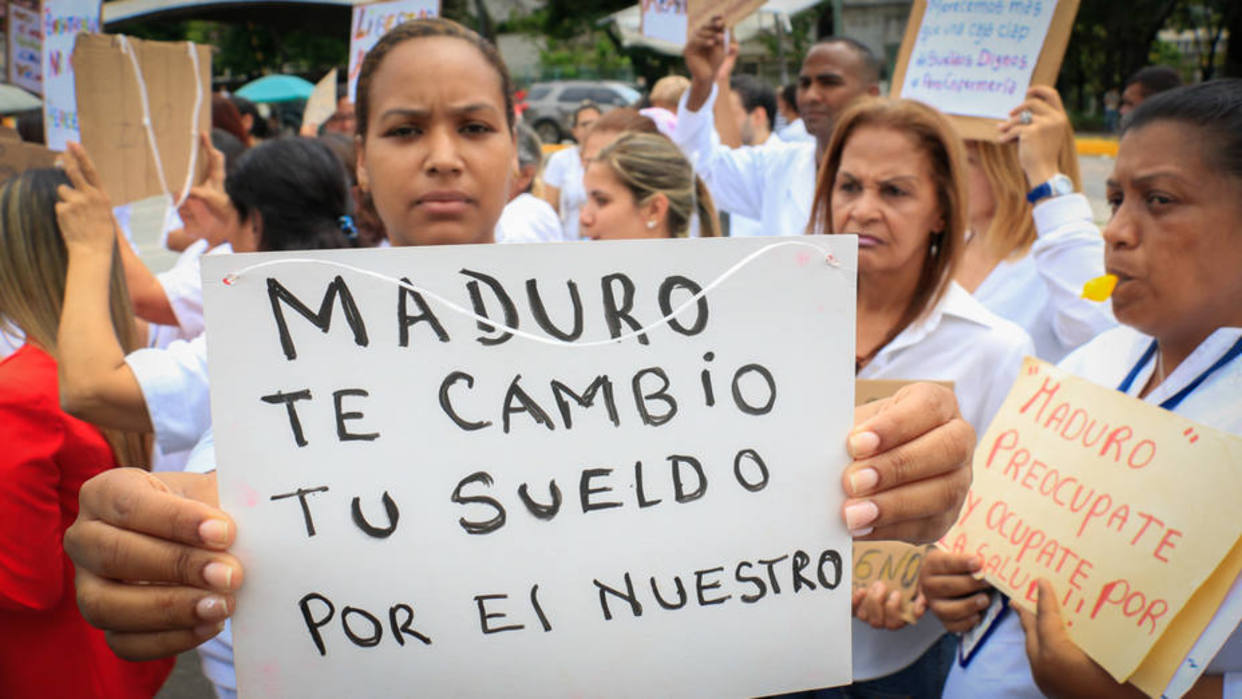
\includegraphics[width=300px]{12.jpg}%
\newline%
%
El Observatorio Venezolano de Conflictividad Social documentó con 983 protestas el descontento creciente de los venezolanos. El informe de~la ONG~correspondiente a septiembre señala que se reportaron en promedio 33 protestas diarias, 300\% más que las ocurridas en el mismo mes del año 2017. Del total 87\% de las manifestaciones estuvo determinada por la exigencia de los derechos económicos, sociales, culturales y ambientales, “lo cual quiere decir que la población se siente indefensa al no poder satisfacer sus necesidades básicas”, indicó el estudio.%
\newline%
%
“El Estado debe cumplir con sus obligaciones y atender las demandas de los ciudadanos, priorizar los recursos para el acceso inmediato al derecho a la salud y a la alimentación, generar una política pública de inclusión para todos los ciudadanos, no solo de un sector ideológicamente identificado con el partido oficialista”, advirtió~la ONG~que puntualizó que el extendido estado de excepción y emergencia económica no se ha traducido en recuperación, sino en más controles y poder del Ejecutivo. “Se agudiza la emergencia humanitaria compleja que atraviesa Venezuela”, subrayó.%
\newline%
%
Los derechos laborales volvieron a ser, con mayor fuerza, las principales causas del descontento durante el mes, al registrarse 409 protestas en el país, en las cuales se exigió el respeto a las contrataciones colectivas que el gobierno desconoció con el “paquetazo de Maduro”. No solo los trabajadores públicos dejaron de percibir seguros privados, primas y otros beneficios, sino que también otros sectores se declararon en conflicto. Los profesionales de la salud superaron los 90 días de protesta con al menos 140 acciones de calle, por salarios dignos, insumos médicos, condiciones sanitarias e infraestructura adecuada para la atención de pacientes. A este sector se sumaron los gremios de educación, eléctrico, telecomunicaciones, siderúrgico, entre otros. Los pensionados también manifestaron en 97 oportunidades por la falta de pago completo de sus beneficios.%
\newline%
%
Los servicios públicos repitieron como la segunda causa más frecuente del descontento ciudadano. Un total de 272 protestas, 9 diarias, se registraron por el deterioro de los servicios básicos, entre estos el gas doméstico (125), agua potable (91) y energía eléctrica (56). La alimentación fue otro de los motivos: 44 protestas aproximadamente fueron documentadas en Distrito Capital y estados del sur. “Avanza el colapso”, aseguró~la ONG~y reiteró que 2018 será el año con mayor número de protestas registradas en los últimos 10 años.%
\newline%
%
\end{document}